\section{Introduction}

Language models map hidden states to vocabulary logits through the final
unembedding matrix, or LM head; we call this interface the \emph{readout}.
Lens-style methods decode hidden states into vocabulary distributions, top-token
summaries, prompted continuations, or natural-language descriptions
\citep{nostalgebraist2020,belrose2023tuned,ghandeharioun2024patchscopes}, but
their scores remain atomic: they show which token or contrast is favored, not
which readout directions support, oppose, or ignore that selected score.

\begin{figure}[H]
    \centering
    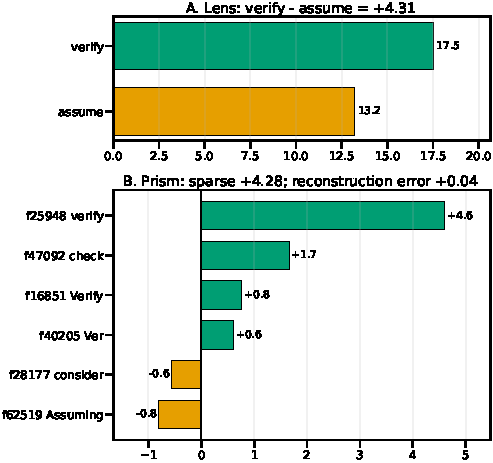
\includegraphics[width=0.92\columnwidth]{figures/proto_token_lens/qwen2b_lens_prism_comparison_verify_assume/qwen2b_lens_prism_comparison_verify_assume.pdf}
    \caption{\textbf{From lens output to a local score account.}
    A logit lens reports a \texttt{verify}-over-\texttt{assume} preference.
    SRP decomposes the same 4.31-logit target into sparse support, opposition,
    and a 0.04-logit reconstruction error.}
    \label{fig:main-lens-prism-comparison}
\end{figure}

Sparse Readout Prism (SRP) turns such scores into calibrated local accounts. It
factorizes unembedding rows with a sparse autoencoder (SAE), giving shared
readout directions and sparse token-row coefficients. A hidden state is first
profiled against these directions; selecting a scalar target---a token logit,
reference contrast, pairwise logit difference, group contrast, or competitor
margin---then yields signed sparse-feature terms and reconstruction error. The
target specifies the question, while reconstruction error and sign agreement
indicate when the sparse account is faithful.

SRP contributes:
\begin{itemize}
    \item a sparse readout basis over unembedding rows, supporting both
    LM-head replacement and target-independent hidden-state profiles.
    \item scalar readout targets and local score accounts for token logits,
    centered logits, logit differences, group contrasts, and local margins.
    \item calibration with replacement quality, target
    reconstruction, sign agreement, and null/reference baselines across a
    multi-family model suite.
    \item demonstrations that target choice changes signed support, context
    reweights profiles, DLA decomposes feature terms, and constrained readout
    edits move held-out lexical scores.
\end{itemize}
